% !TeX root = thesis.tex
\documentclass{master_thesis}

\begin{document}



\appendix
% \section*{Appendices}
% \addcontentsline{toc}{section}{Appendices}
\section{Pre-case study questionnaire }\label{appendix:pre-survey}
\subsection{Pre-case study questionnaire questions}\label{appendix:pre-survey-questions}
\subsection{Pre-case study questionnaire replies}\label{appendix:pre-survey-replies}
\section{Post-case study questionnaire }\label{appendix:post-survey}
\subsection{Post-case study questionnaire questions}\label{appendix:post-survey-questions}
\subsection{Post-case study questionnaire replies}\label{appendix:post-survey-replies}
\section{Accessibility report}\label{appendix:report}

% 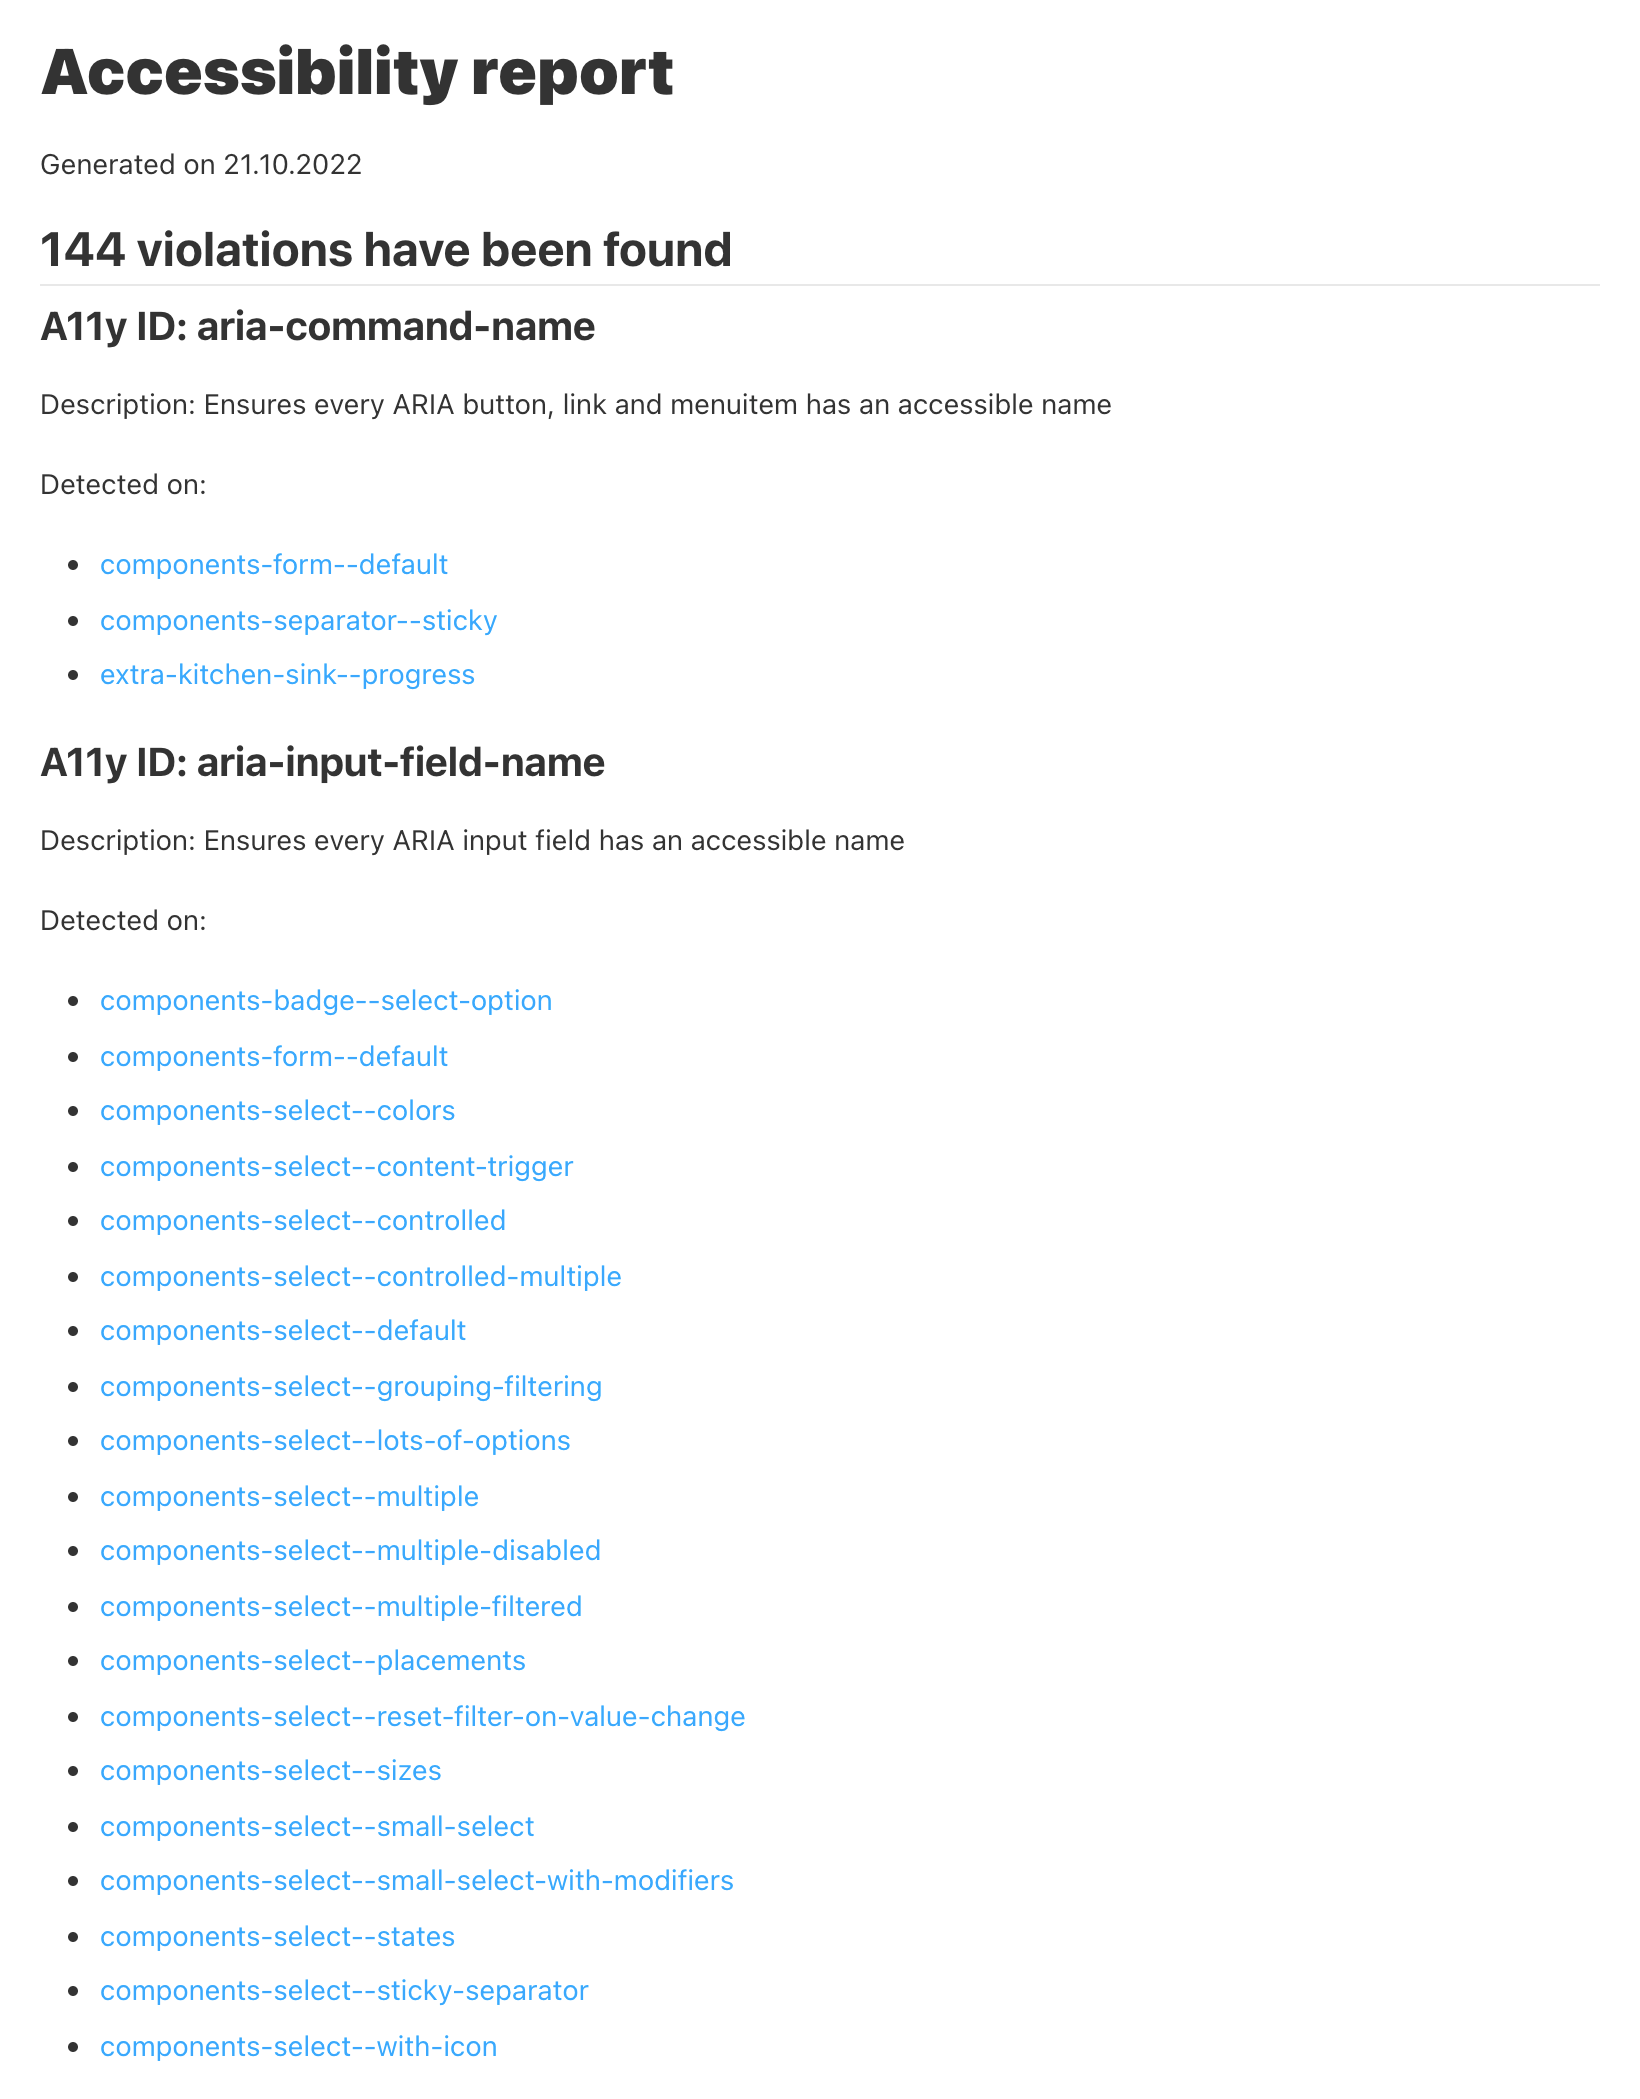
\includegraphics[width=\textwidth]{img/report/a11y-report-1.png}
% 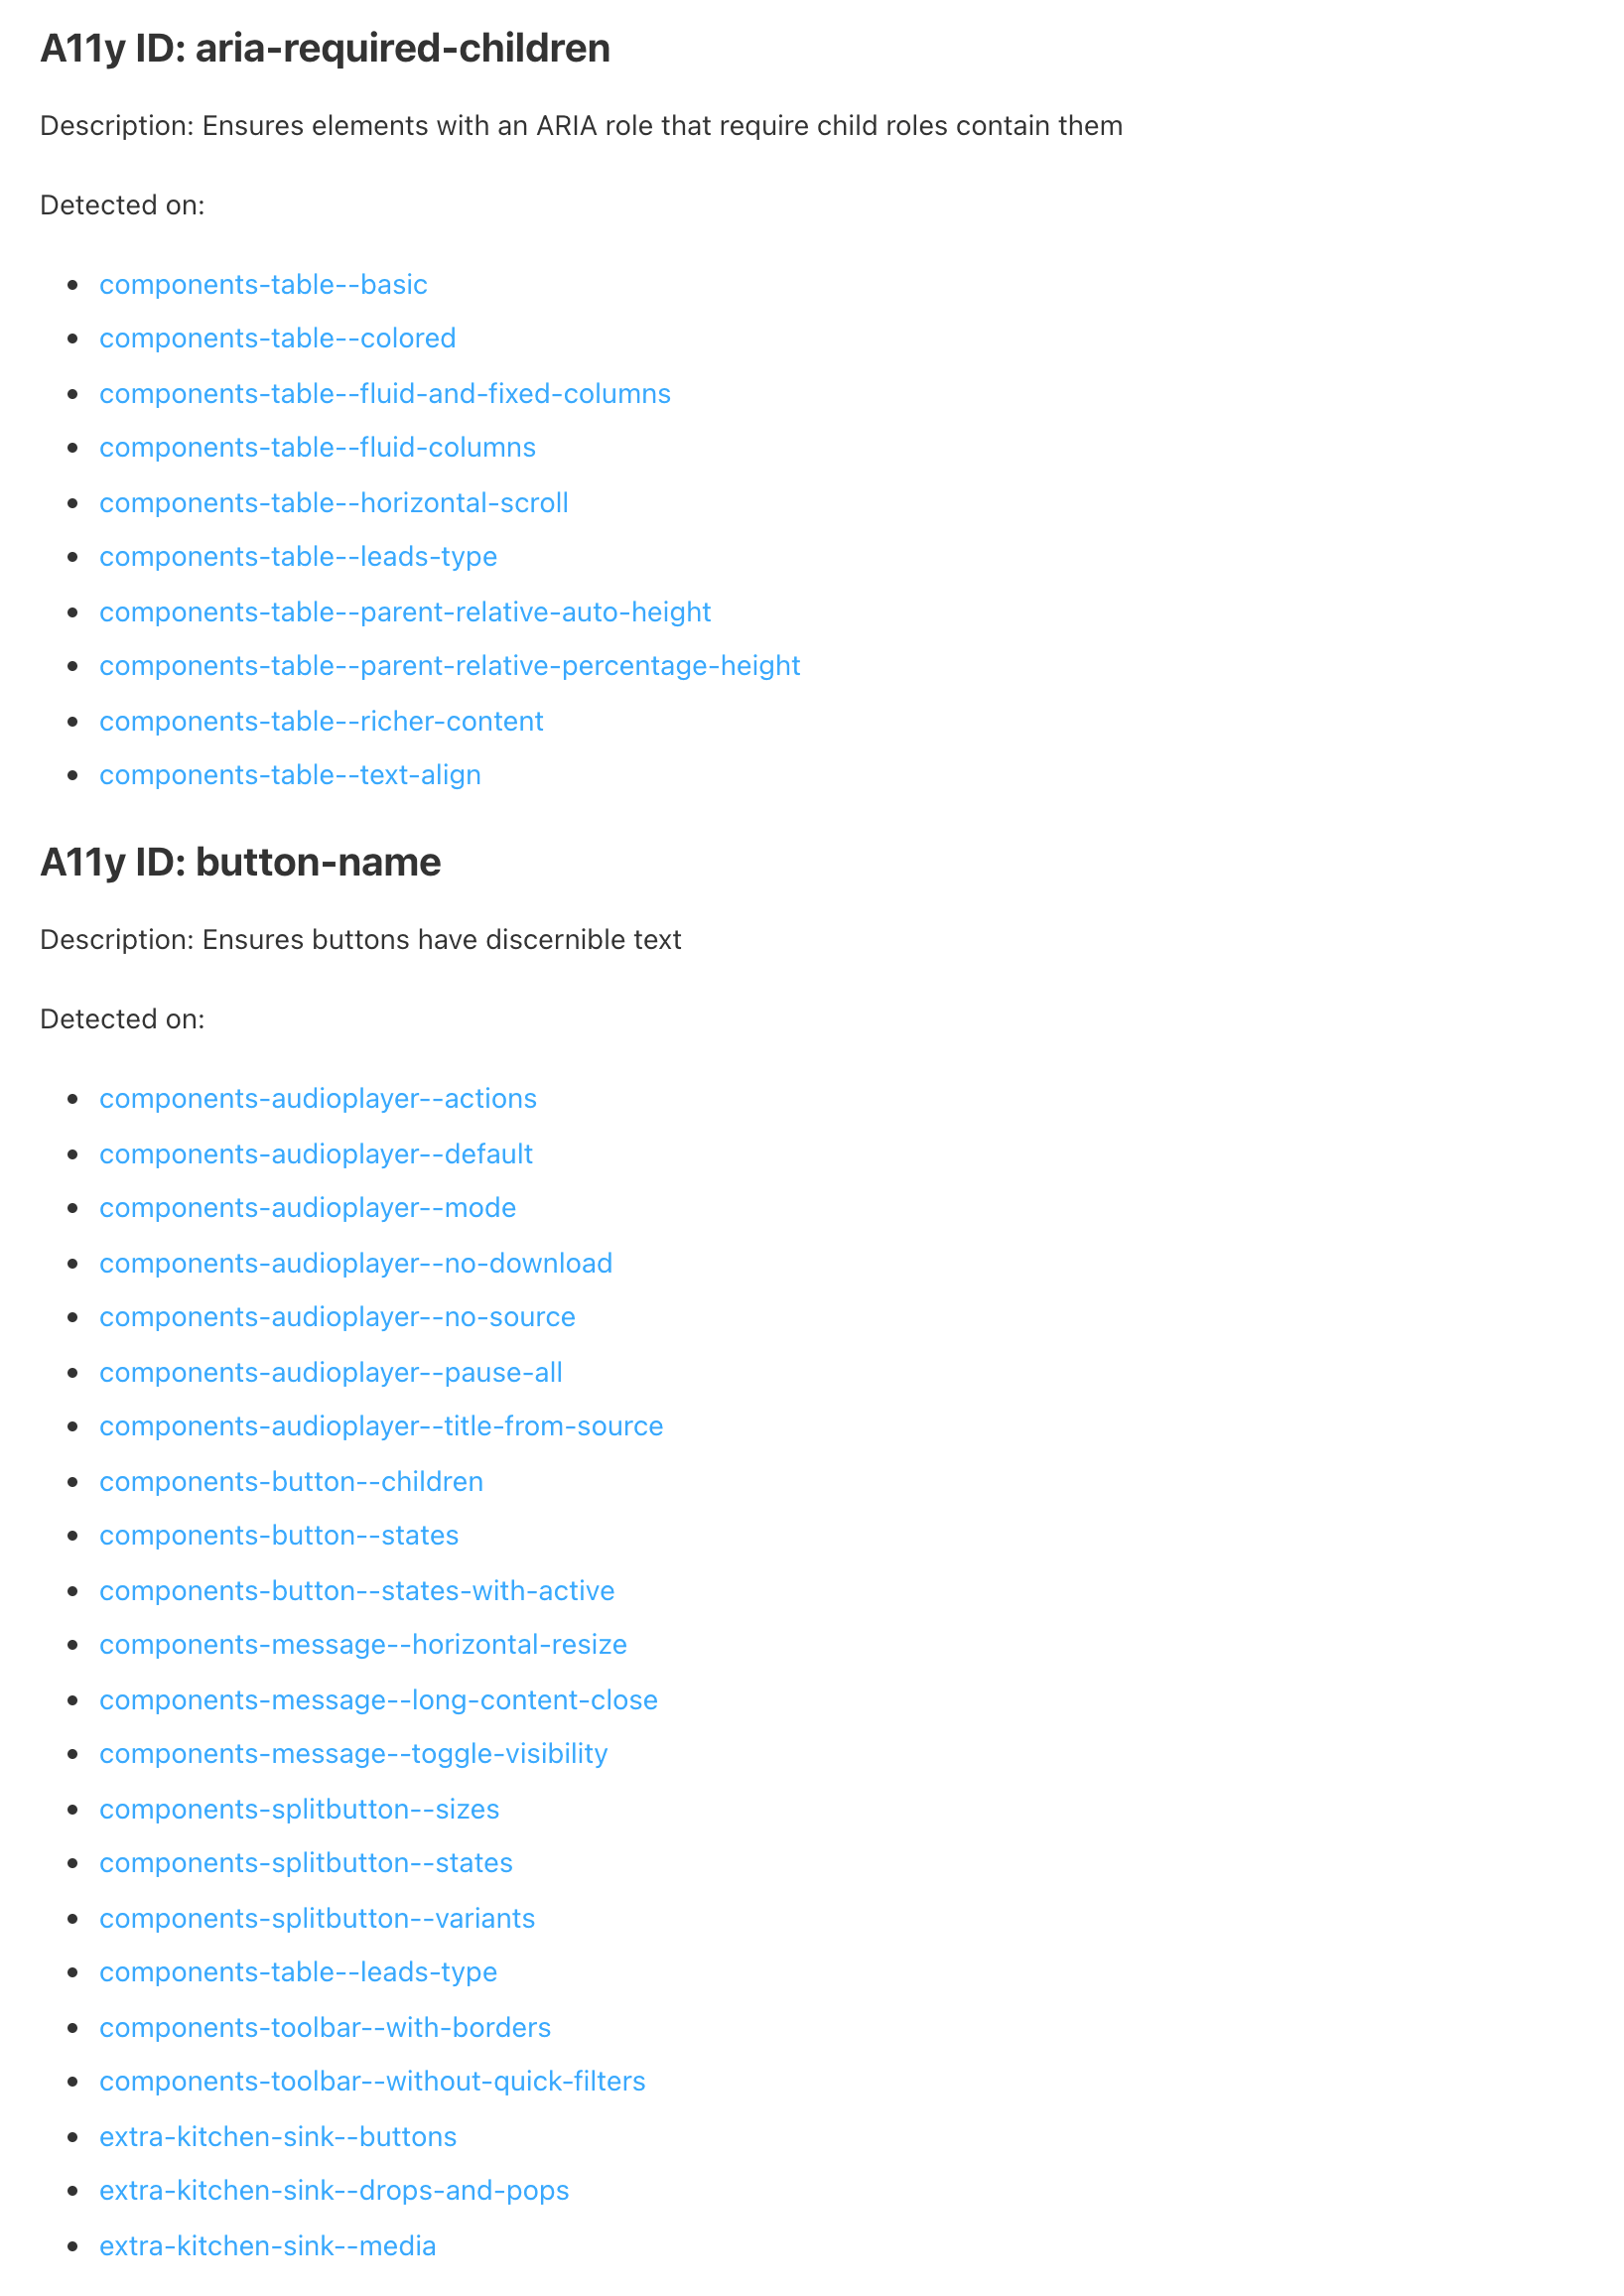
\includegraphics[width=\textwidth]{img/report/a11y-report-2.png}
% 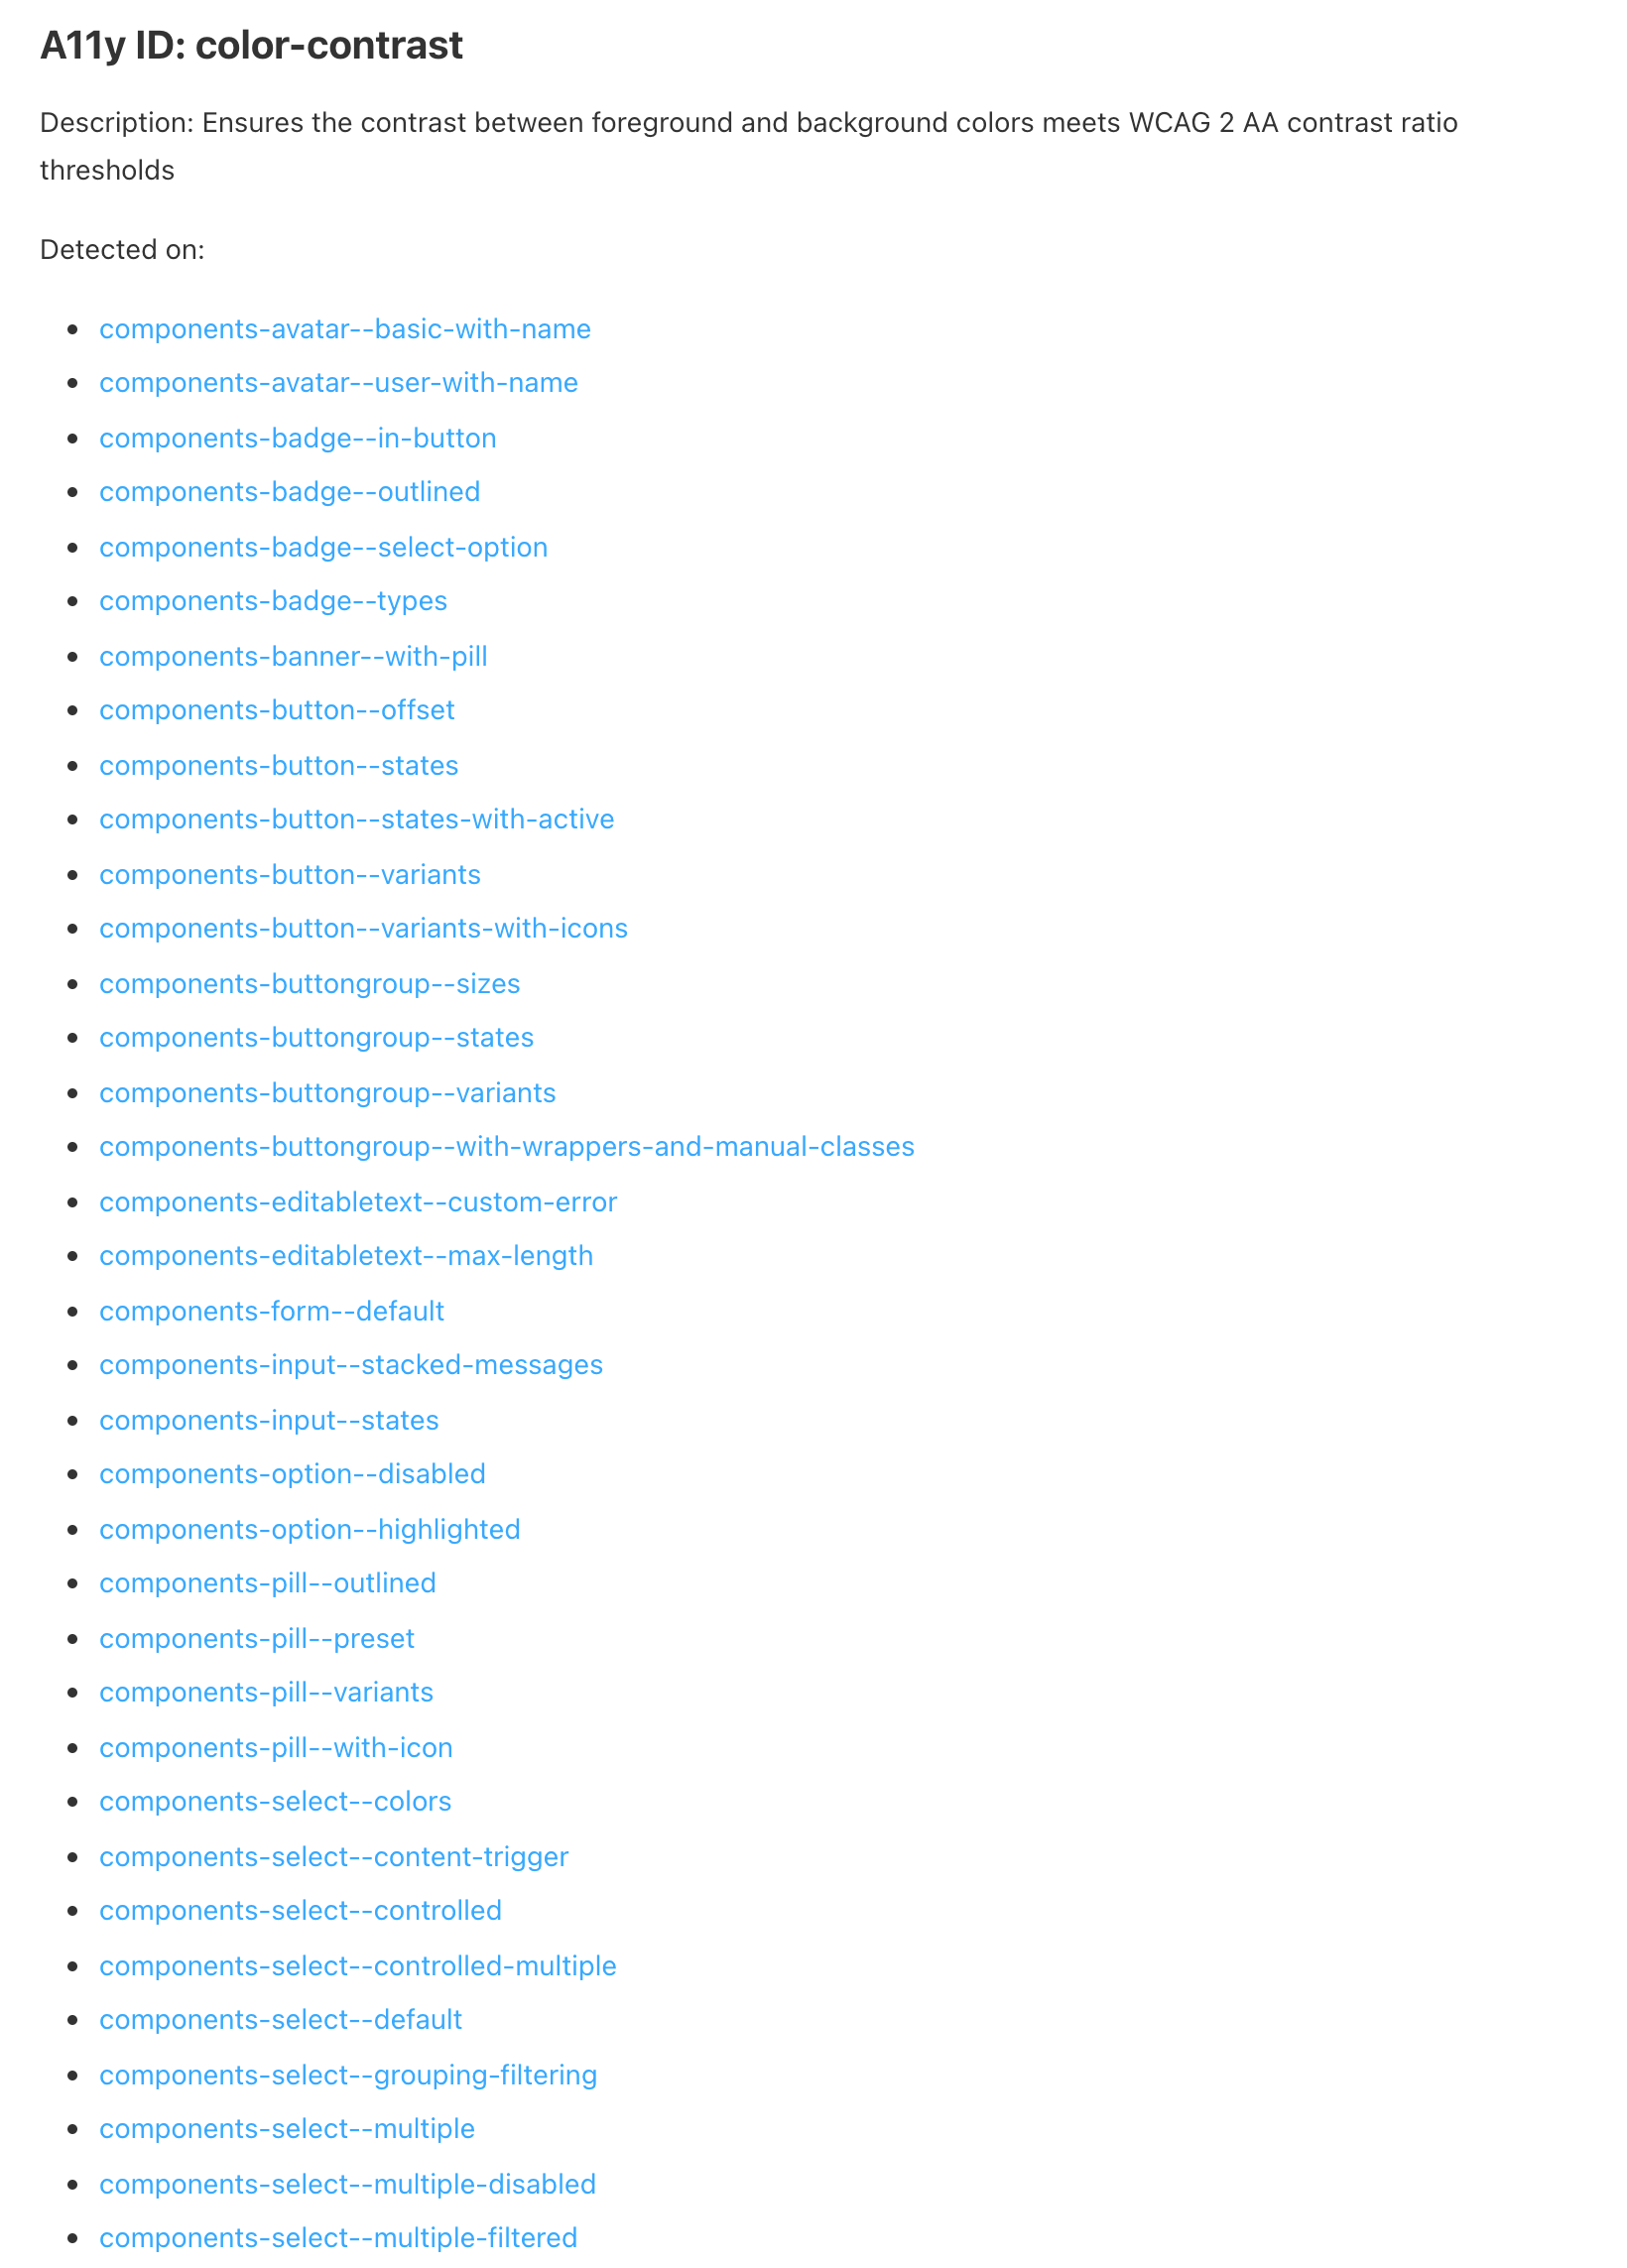
\includegraphics[width=\textwidth]{img/report/a11y-report-3.png}
% 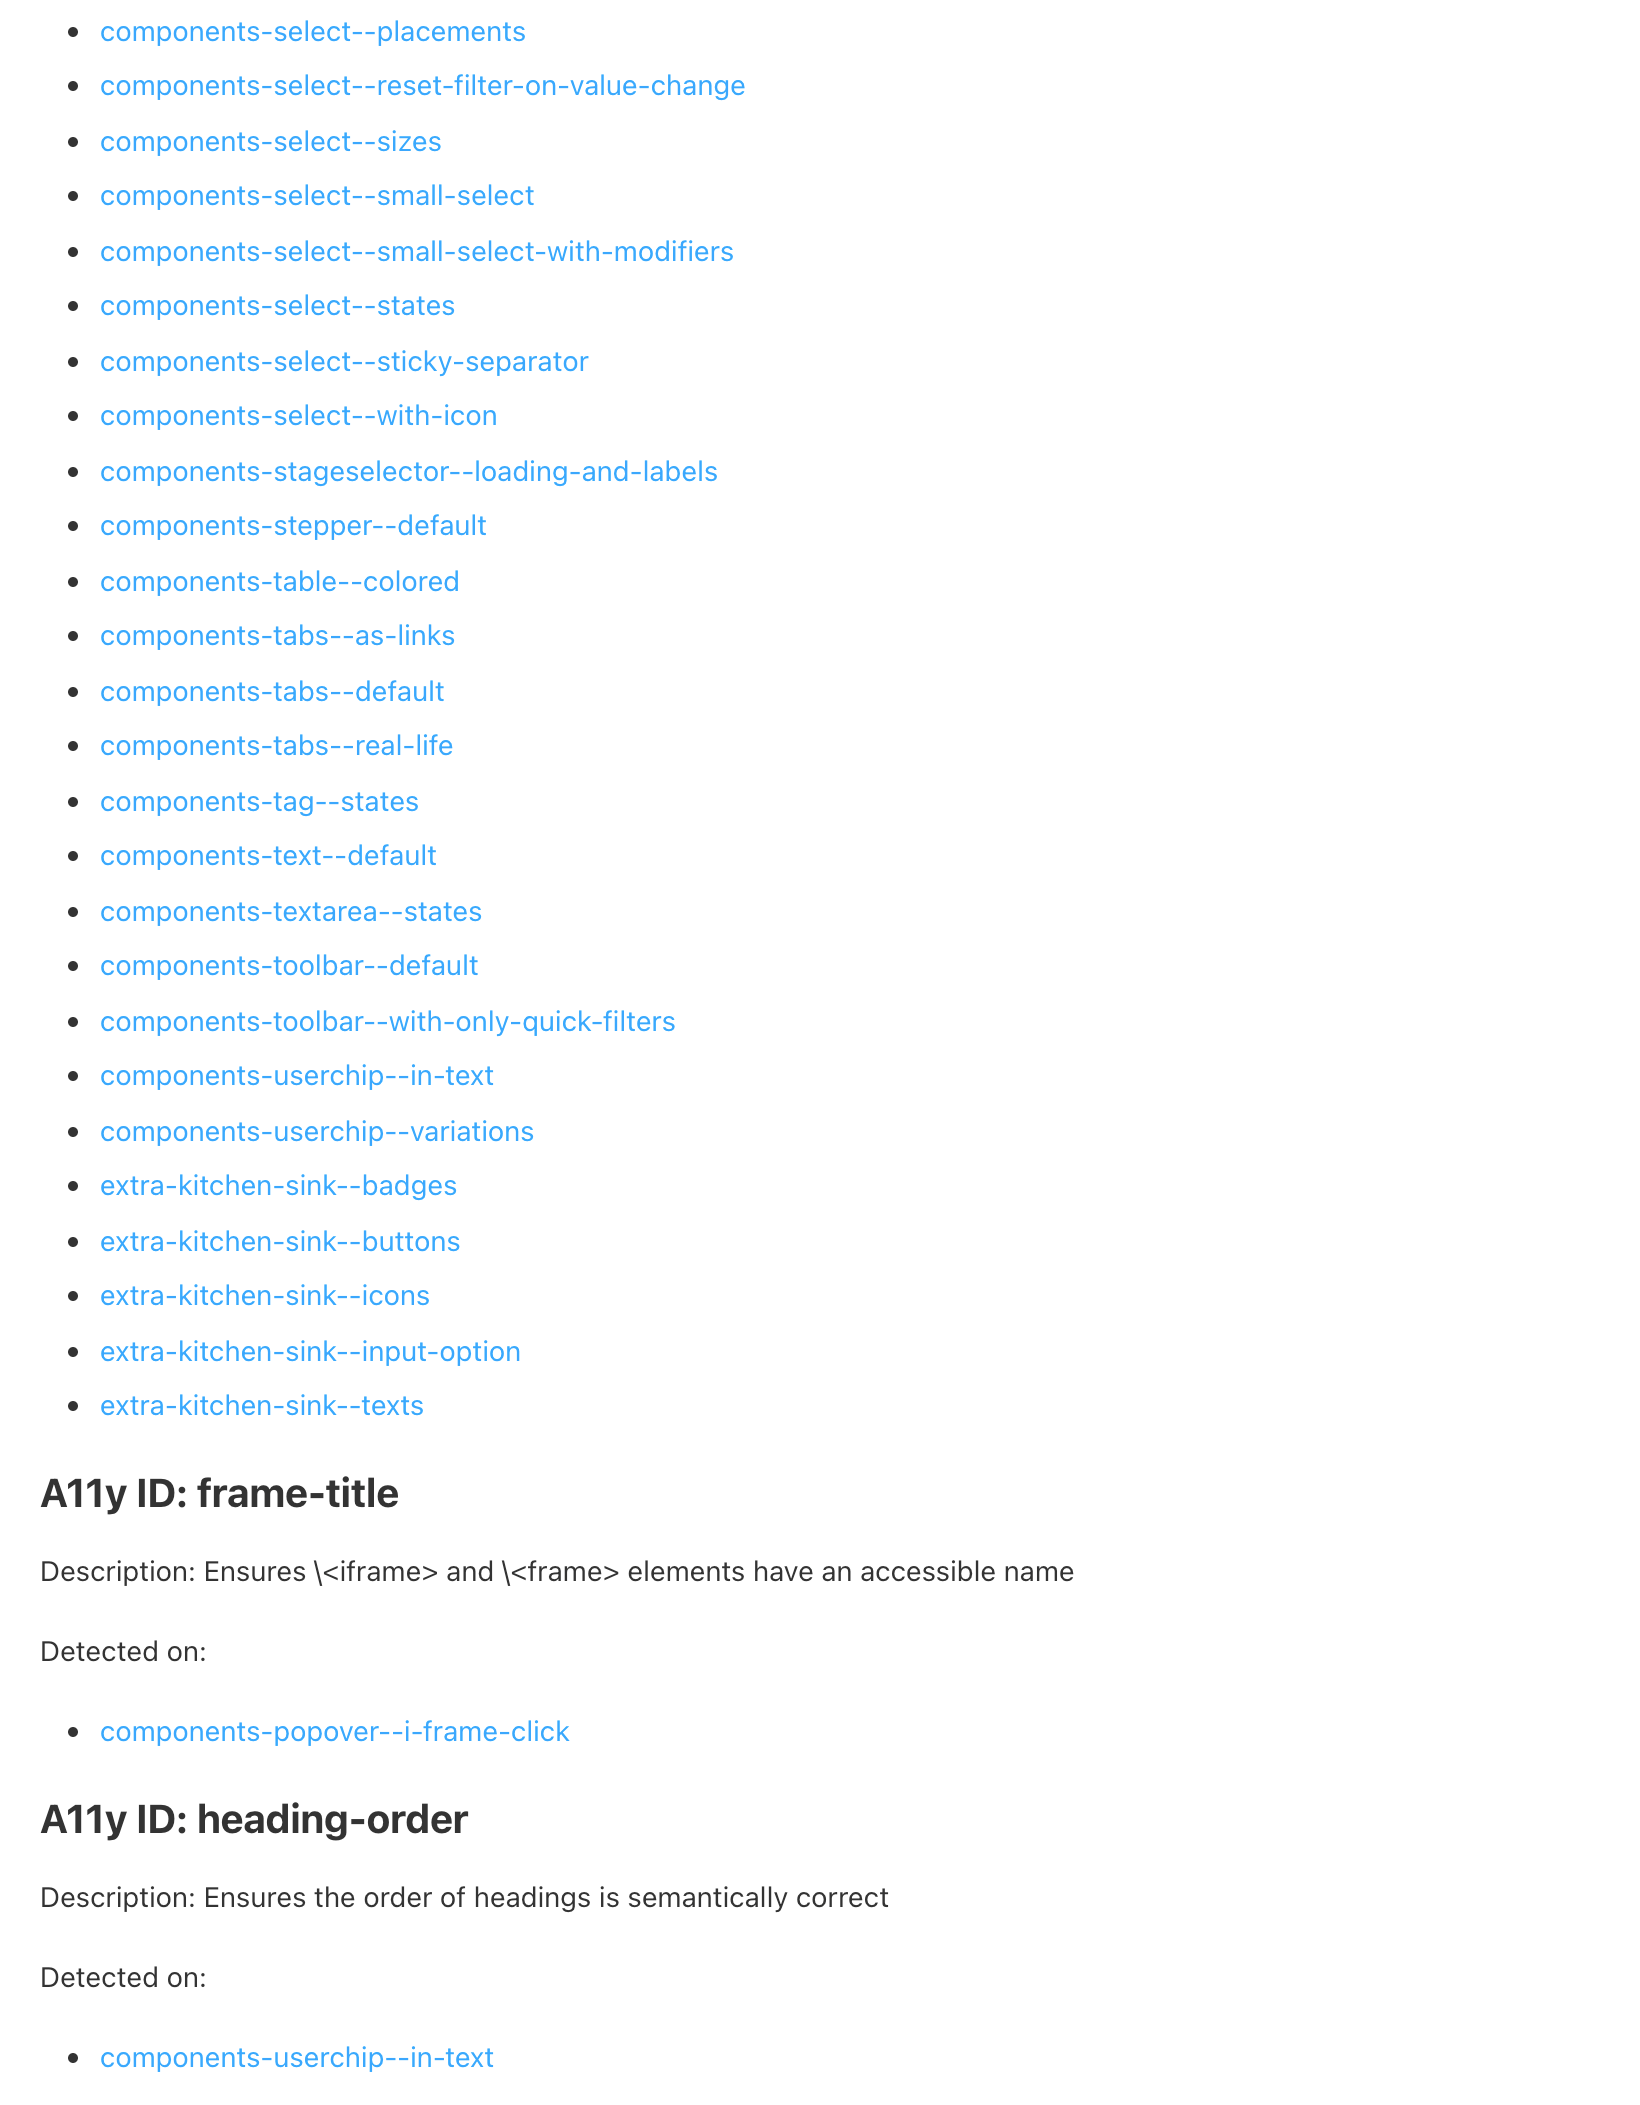
\includegraphics[width=\textwidth]{img/report/a11y-report-4.png}
% 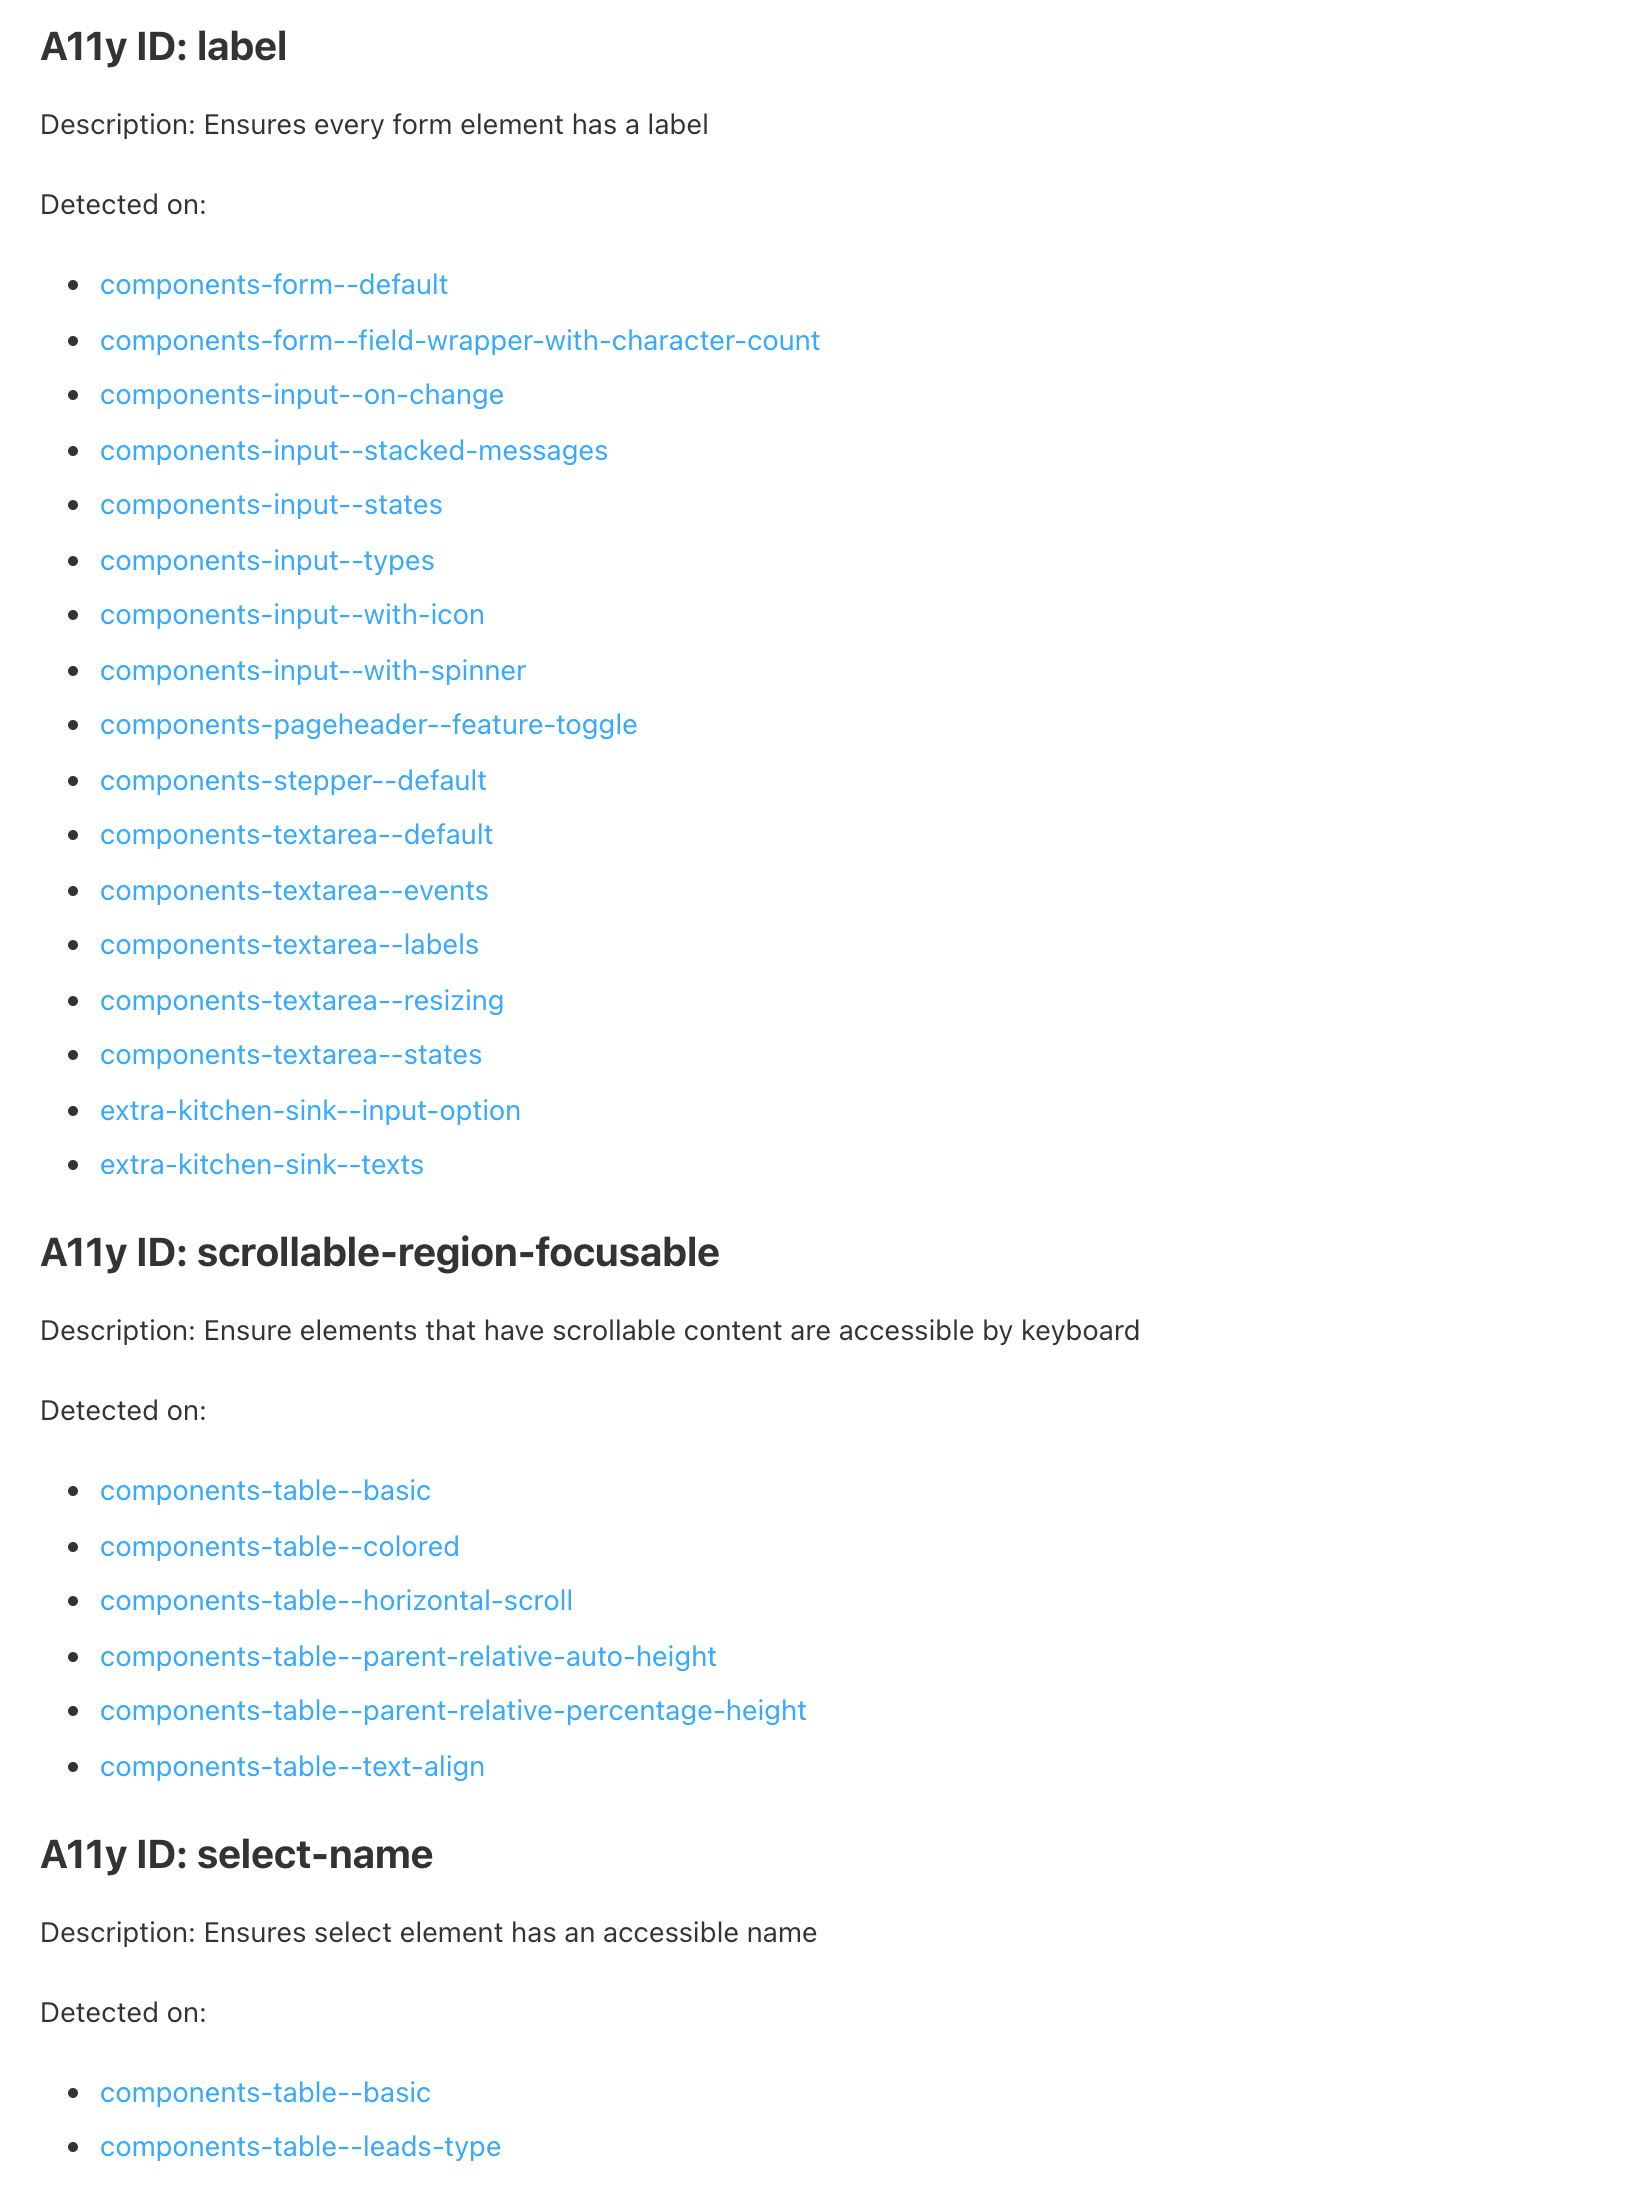
\includegraphics[width=\textwidth]{img/report/a11y-report-5.png}

\section{Manual Accessibility audit results}\label{appendix:manual-audit}

\section{Table of summarized accessibility test results}\label{appendix:results-table}

\todo{add automated test report, manual testing report and the comparison between them here}

\begin{table}[!ht]
    \centering
    \begin{tabular}{|l|l|l|l|l|l|l|l|l|l|l|l|l|}
    \hline
        Component & fail & fail(valid) & diff & pass & pass(valid) & pass+fail & diff & manual  \\ \hline
        AudioPlayer & 8 & 3 & 5 & 2 & 2 & 10 & 0 & 3  \\ \hline
        Avatar & 2 & 2 & 0 & 0 & 0 & 2 & 0 & 0  \\ \hline
        BabyPill & 0 & 0 & 0 & 4 & 0 & 4 & 4 & 1  \\ \hline
        Badge & 5 & 4 & 1 & 10 & 1 & 15 & 9 & 0  \\ \hline
        Banner & 1 & 0 & 1 & 4 & 4 & 5 & 0 & 0  \\ \hline
        Button & 12 & 4 & 8 & 4 & 3 & 16 & 1 & 2  \\ \hline
        ButtonGroup & 4 & 2 & 2 & 0 & 0 & 4 & 0 & 2  \\ \hline
        Checkbox & 0 & 0 & 0 & 5 & 5 & 5 & 0 & 2  \\ \hline
        Coachmark & 0 & 0 & 0 & 3 & 0 & 3 & 3 & 3  \\ \hline
        Dialog & 0 & 0 & 0 & 3 & 0 & 3 & 3 & 3  \\ \hline
        Divider & 0 & 0 & 0 & 6 & 0 & 6 & 6 & 0  \\ \hline
        Dropmenu & 0 & 0 & 0 & 3 & 0 & 3 & 3 & 0  \\ \hline
        EditableText & 2 & 1 & 1 & 7 & 7 & 9 & 0 & 1  \\ \hline
        FeedbackModal & 0 & 0 & 0 & 3 & 0 & 3 & 3 & 1  \\ \hline
        Form & 5 & 3 & 2 & 18 & 17 & 23 & 1 & 1  \\ \hline
        Icon & 0 & 0 & 0 & 1 & 0 & 1 & 1 & 0  \\ \hline
        IconButton & 0 & 0 & 0 & 5 & 5 & 5 & 0 & 2  \\ \hline
        ImageOverlay & 0 & 0 & 0 & 3 & 0 & 3 & 3 & 4  \\ \hline
        InlineInfo & 0 & 0 & 0 & 5 & 5 & 5 & 0 & 1  \\ \hline
    \end{tabular}
\end{table}



\end{document}